\section{User Manual}

\subsection{Overview}
When the application is started the user can choose between three features.
\begin{itemize}
  \item Creating a new task
  \item Showing all tasks
  \item Modify the settings
\end{itemize}
 \begin{figure}[h]
  \caption{Main screen}
  \center
  	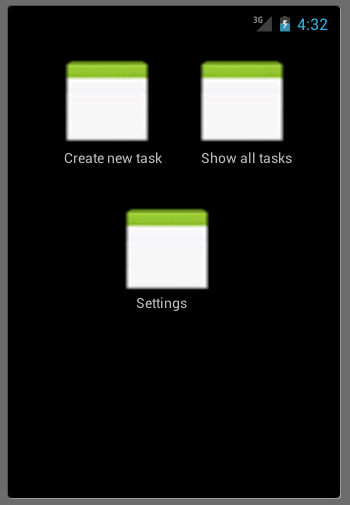
\includegraphics[scale=0.25]{../resources/main.png}
\end{figure}

\subsection{Creating a task}
In order to create a new task the user has to assign the \emph{task name}, a
\emph{task description} and link it to a \emph{location}. Google Maps is used to
assist the user with the search for a location.
 \begin{figure}[h]
  \caption{Choosing a location}
  \center
  	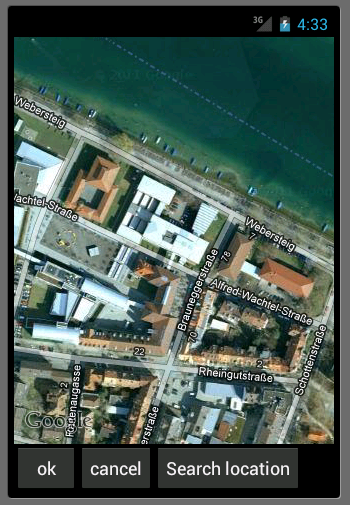
\includegraphics[scale=0.25]{../resources/choose-location.png}
\end{figure}
The user has the ability to link his task to a time span. This feature will
ensure, that the user is not only reminded when he is in range of the given
location point, but also when the current time matches the specified time span.
In case the time span is not explicitly specified, the application defaults to
always reminding the user. The user might also assign an urgency indicator to a
task. The urgency will be represented by a color code. There are three urgency
states: \emph{high}, \emph{middle} and \emph{low}, represented by
\textcolor{red}{red}, \textcolor{yellow}{yellow} and \textcolor{green}{green}
colors respectively.
 \begin{figure}[h]
  \caption{Creating a task}
  \center
  	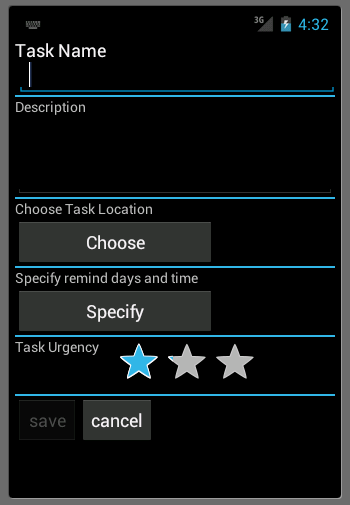
\includegraphics[scale=0.25]{../resources/create-task.png}
\end{figure}

\subsection{Showing all available tasks}
All tasks are shown in a simple list. The urgency is represented by a
vertical colored line on the left side of the icon. The icon indicates the status of a
given to-do task. The user can press one of the items so a further menu is
displayed. The menu contains features described in the following sections.
 \begin{figure}[h]
  \caption{Showing all available tasks}
  \center
  	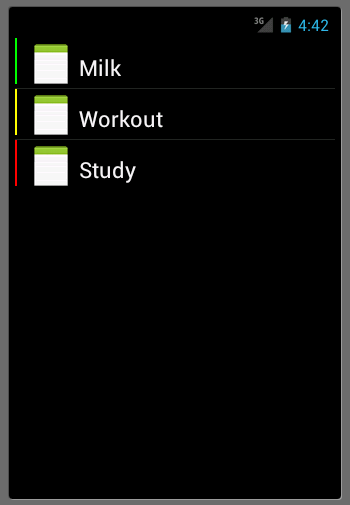
\includegraphics[scale=0.25]{../resources/show-all-tasks.png}
\end{figure}

\subsection{Editing a task}
The \emph{edit task} feature is available from the \emph{show all tasks} screen.
In order to edit a task the user has to select the desired task by touching it.
The menu is inflated and the \emph{edit task} item has to be selected.
\newline
\newline
The screen shown to the user is identical to the screen he already
knows from the \emph{create task} feature. This time all predefined fields are
already filled in and their content may be altered as desired.
 \begin{figure}[h]
  \caption{Editing a task}
  \center
  	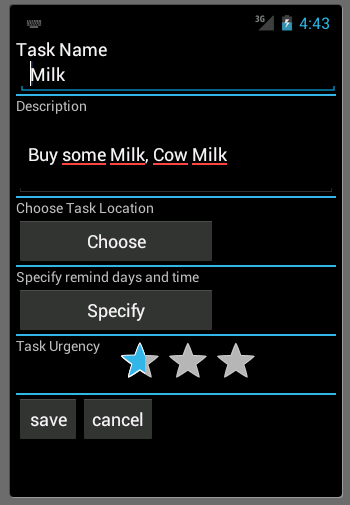
\includegraphics[scale=0.25]{../resources/edit-task.png}
\end{figure}

\subsection{Deleting a task}
The \emph{delete task} feature is also available from the \emph{show all tasks}
screen. In order to delete a task the user has to select the desired task by
touching it. The menu is inflated and the \emph{delete task} item has to be
selected. After the task has been deleted the user is redirected to the
\emph{show all tasks} screen.
 \begin{figure}[h]
  \caption{Item menu}
  \center
  	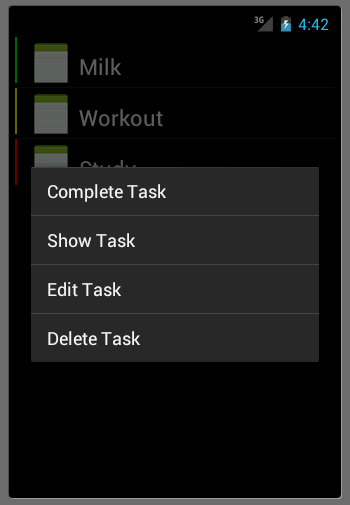
\includegraphics[scale=0.25]{../resources/item-menu.png}
\end{figure}

\subsection{Solving a task}
The \emph{solve task} feature is also available from the \emph{show all tasks}
screen. In order to complete a task the user has to select the
desired task by touching it. The menu is inflated and the \emph{complete task}
item has to be selected. After the task has been completed the user is
redirected to the \emph{show all tasks} screen. This time the icon of the task
is altered. The icon generally indicates the status of the task.
The status is restored to \emph{unsolved} after the task has been edited.
 \begin{figure}[h]
  \caption{Completed task}
  \center
  	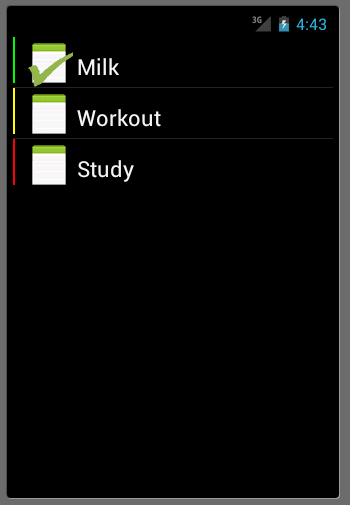
\includegraphics[scale=0.25]{../resources/completed-task.png}
\end{figure}

\subsection{Showing a task}
The \emph{show task} feature displays the details of the given tasks. It is also
available from the \emph{show all tasks} screen. In order to show a task the
user has to select the desired task by touching it. The menu is inflated and the
\emph{show task} item has to be selected. The following figure shows the
representation of the task.
 \begin{figure}[h]
  \caption{Showing a task}
  \center
  	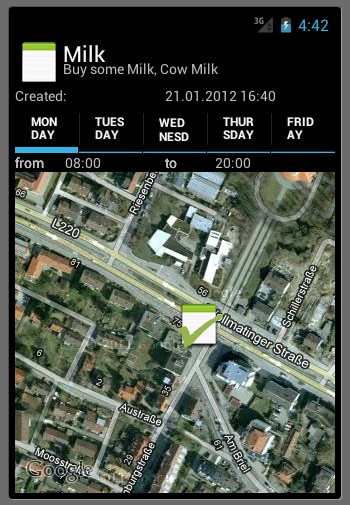
\includegraphics[scale=0.25]{../resources/show-task.png}
\end{figure}

\subsection{Configuring the application}
The user has the ability to configure the following options:
\begin{itemize}
  \item Setting the reminding radius
  \item Setting the update frequency
  \item Adjusting the reminding mode
\end{itemize}
 \begin{figure}[h]
  \caption{Settings screen}
  \center
  	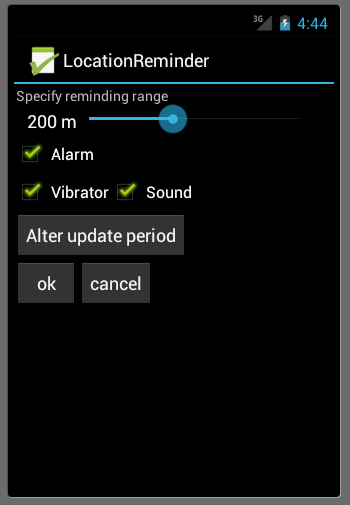
\includegraphics[scale=0.25]{../resources/preferences-view.png}
\end{figure}

\subsubsection{Setting the reminding radius}
The radius specifies the number of meters from the current position to the
linked to-do item. The radius has to be in range from 0 up to 500 meters. A
horizontal scrollbar makes sure that the user stays within this range.

\subsubsection{Setting the update frequency}
A service runs in the background of the application, which provides the current
position of the smartphone. The user has the ability to specify the frequency of
how often this service updates its data. The user may pick one of the many
options, spanning from 1 minute up to 24 hours, represented by a drop-down list.

\subsubsection{Adjusting the reminding mode}
The reminder can be turned on and off. The user may select the way he wants to
be reminded when the reminder is on. The options are \emph{ring-alarm},
\emph{vibration} or both.
